% Options for packages loaded elsewhere
\PassOptionsToPackage{unicode}{hyperref}
\PassOptionsToPackage{hyphens}{url}
%
\documentclass[
]{article}
\usepackage{lmodern}
\usepackage{amssymb,amsmath}
\usepackage{ifxetex,ifluatex}
\ifnum 0\ifxetex 1\fi\ifluatex 1\fi=0 % if pdftex
  \usepackage[T1]{fontenc}
  \usepackage[utf8]{inputenc}
  \usepackage{textcomp} % provide euro and other symbols
\else % if luatex or xetex
  \usepackage{unicode-math}
  \defaultfontfeatures{Scale=MatchLowercase}
  \defaultfontfeatures[\rmfamily]{Ligatures=TeX,Scale=1}
\fi
% Use upquote if available, for straight quotes in verbatim environments
\IfFileExists{upquote.sty}{\usepackage{upquote}}{}
\IfFileExists{microtype.sty}{% use microtype if available
  \usepackage[]{microtype}
  \UseMicrotypeSet[protrusion]{basicmath} % disable protrusion for tt fonts
}{}
\makeatletter
\@ifundefined{KOMAClassName}{% if non-KOMA class
  \IfFileExists{parskip.sty}{%
    \usepackage{parskip}
  }{% else
    \setlength{\parindent}{0pt}
    \setlength{\parskip}{6pt plus 2pt minus 1pt}}
}{% if KOMA class
  \KOMAoptions{parskip=half}}
\makeatother
\usepackage{xcolor}
\IfFileExists{xurl.sty}{\usepackage{xurl}}{} % add URL line breaks if available
\IfFileExists{bookmark.sty}{\usepackage{bookmark}}{\usepackage{hyperref}}
\hypersetup{
  hidelinks,
  pdfcreator={LaTeX via pandoc}}
\urlstyle{same} % disable monospaced font for URLs
\usepackage[margin=1in]{geometry}
\usepackage{color}
\usepackage{fancyvrb}
\newcommand{\VerbBar}{|}
\newcommand{\VERB}{\Verb[commandchars=\\\{\}]}
\DefineVerbatimEnvironment{Highlighting}{Verbatim}{commandchars=\\\{\}}
% Add ',fontsize=\small' for more characters per line
\usepackage{framed}
\definecolor{shadecolor}{RGB}{248,248,248}
\newenvironment{Shaded}{\begin{snugshade}}{\end{snugshade}}
\newcommand{\AlertTok}[1]{\textcolor[rgb]{0.94,0.16,0.16}{#1}}
\newcommand{\AnnotationTok}[1]{\textcolor[rgb]{0.56,0.35,0.01}{\textbf{\textit{#1}}}}
\newcommand{\AttributeTok}[1]{\textcolor[rgb]{0.77,0.63,0.00}{#1}}
\newcommand{\BaseNTok}[1]{\textcolor[rgb]{0.00,0.00,0.81}{#1}}
\newcommand{\BuiltInTok}[1]{#1}
\newcommand{\CharTok}[1]{\textcolor[rgb]{0.31,0.60,0.02}{#1}}
\newcommand{\CommentTok}[1]{\textcolor[rgb]{0.56,0.35,0.01}{\textit{#1}}}
\newcommand{\CommentVarTok}[1]{\textcolor[rgb]{0.56,0.35,0.01}{\textbf{\textit{#1}}}}
\newcommand{\ConstantTok}[1]{\textcolor[rgb]{0.00,0.00,0.00}{#1}}
\newcommand{\ControlFlowTok}[1]{\textcolor[rgb]{0.13,0.29,0.53}{\textbf{#1}}}
\newcommand{\DataTypeTok}[1]{\textcolor[rgb]{0.13,0.29,0.53}{#1}}
\newcommand{\DecValTok}[1]{\textcolor[rgb]{0.00,0.00,0.81}{#1}}
\newcommand{\DocumentationTok}[1]{\textcolor[rgb]{0.56,0.35,0.01}{\textbf{\textit{#1}}}}
\newcommand{\ErrorTok}[1]{\textcolor[rgb]{0.64,0.00,0.00}{\textbf{#1}}}
\newcommand{\ExtensionTok}[1]{#1}
\newcommand{\FloatTok}[1]{\textcolor[rgb]{0.00,0.00,0.81}{#1}}
\newcommand{\FunctionTok}[1]{\textcolor[rgb]{0.00,0.00,0.00}{#1}}
\newcommand{\ImportTok}[1]{#1}
\newcommand{\InformationTok}[1]{\textcolor[rgb]{0.56,0.35,0.01}{\textbf{\textit{#1}}}}
\newcommand{\KeywordTok}[1]{\textcolor[rgb]{0.13,0.29,0.53}{\textbf{#1}}}
\newcommand{\NormalTok}[1]{#1}
\newcommand{\OperatorTok}[1]{\textcolor[rgb]{0.81,0.36,0.00}{\textbf{#1}}}
\newcommand{\OtherTok}[1]{\textcolor[rgb]{0.56,0.35,0.01}{#1}}
\newcommand{\PreprocessorTok}[1]{\textcolor[rgb]{0.56,0.35,0.01}{\textit{#1}}}
\newcommand{\RegionMarkerTok}[1]{#1}
\newcommand{\SpecialCharTok}[1]{\textcolor[rgb]{0.00,0.00,0.00}{#1}}
\newcommand{\SpecialStringTok}[1]{\textcolor[rgb]{0.31,0.60,0.02}{#1}}
\newcommand{\StringTok}[1]{\textcolor[rgb]{0.31,0.60,0.02}{#1}}
\newcommand{\VariableTok}[1]{\textcolor[rgb]{0.00,0.00,0.00}{#1}}
\newcommand{\VerbatimStringTok}[1]{\textcolor[rgb]{0.31,0.60,0.02}{#1}}
\newcommand{\WarningTok}[1]{\textcolor[rgb]{0.56,0.35,0.01}{\textbf{\textit{#1}}}}
\usepackage{graphicx,grffile}
\makeatletter
\def\maxwidth{\ifdim\Gin@nat@width>\linewidth\linewidth\else\Gin@nat@width\fi}
\def\maxheight{\ifdim\Gin@nat@height>\textheight\textheight\else\Gin@nat@height\fi}
\makeatother
% Scale images if necessary, so that they will not overflow the page
% margins by default, and it is still possible to overwrite the defaults
% using explicit options in \includegraphics[width, height, ...]{}
\setkeys{Gin}{width=\maxwidth,height=\maxheight,keepaspectratio}
% Set default figure placement to htbp
\makeatletter
\def\fps@figure{htbp}
\makeatother
\setlength{\emergencystretch}{3em} % prevent overfull lines
\providecommand{\tightlist}{%
  \setlength{\itemsep}{0pt}\setlength{\parskip}{0pt}}
\setcounter{secnumdepth}{-\maxdimen} % remove section numbering

\title{Econometrics III\\
Assignment Part 1 \& 2\\
Tinbergen Insitute}
\author{Stanislav Avdeev \& Bas Machielsen\\
student no \hspace{5m} 590049bm\\
\href{mailto:stnavdeev@gmail.com}{\nolinkurl{stnavdeev@gmail.com}}
\hspace{5m} \href{mailto:590049bm@eur.nl}{\nolinkurl{590049bm@eur.nl}}}
\date{\today}

\begin{document}
\maketitle

\hypertarget{instructions}{%
\subsection{Instructions}\label{instructions}}

I created a file .Renviron, where the python distribution is located on
my system. You can find that by opening a terminal, and entering
\texttt{\$\ which\ -a\ python\ python3}. Then, in RStudio, use
\texttt{usethis::edit\_r\_environ()}, and add
\texttt{RETICULATE\_PYTHON="/Users/basmachielsen/opt/anaconda3/bin/python"}
(or your directory) on a new line to the file. In this way, we can
seamlessly interchange R and Python code chunks. Restart RStudio, and
then everything is ready to go:

\begin{Shaded}
\begin{Highlighting}[]
\KeywordTok{summary}\NormalTok{(cars)}
\end{Highlighting}
\end{Shaded}

\begin{verbatim}
##      speed           dist       
##  Min.   : 4.0   Min.   :  2.00  
##  1st Qu.:12.0   1st Qu.: 26.00  
##  Median :15.0   Median : 36.00  
##  Mean   :15.4   Mean   : 42.98  
##  3rd Qu.:19.0   3rd Qu.: 56.00  
##  Max.   :25.0   Max.   :120.00
\end{verbatim}

\begin{Shaded}
\begin{Highlighting}[]
\NormalTok{mtcars <-}\StringTok{ }\NormalTok{mtcars}
\end{Highlighting}
\end{Shaded}

\begin{Shaded}
\begin{Highlighting}[]
\ImportTok{import}\NormalTok{ pandas }\ImportTok{as}\NormalTok{ pd}
\ImportTok{import}\NormalTok{ numpy }\ImportTok{as}\NormalTok{ np}

\NormalTok{r.mtcars.}\BuiltInTok{sum}\NormalTok{()}
\end{Highlighting}
\end{Shaded}

\begin{verbatim}
## mpg      642.900
## cyl      198.000
## disp    7383.100
## hp      4694.000
## drat     115.090
## wt       102.952
## qsec     571.160
## vs        14.000
## am        13.000
## gear     118.000
## carb      90.000
## dtype: float64
\end{verbatim}

\hypertarget{including-plots}{%
\subsection{Including Plots}\label{including-plots}}

You can also embed plots, for example:

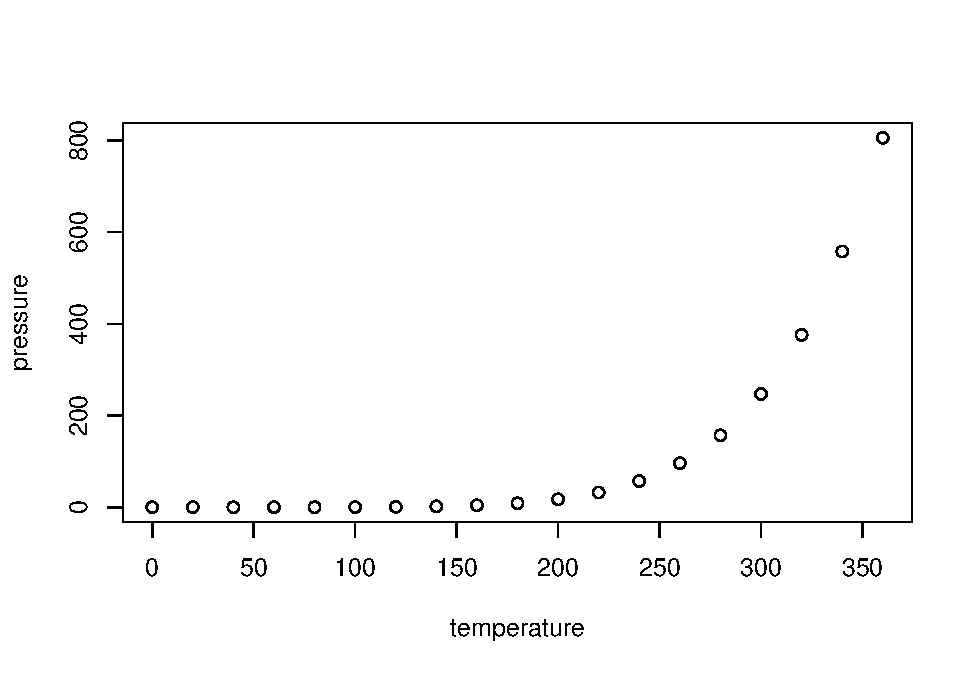
\includegraphics{assignment_1_files/figure-latex/pressure-1.pdf}

Note that the \texttt{echo\ =\ FALSE} parameter was added to the code
chunk to prevent printing of the R code that generated the plot.

\hypertarget{including-matplotlib}{%
\subsection{Including Matplotlib}\label{including-matplotlib}}

\begin{Shaded}
\begin{Highlighting}[]
\NormalTok{hoi }\OperatorTok{=}\NormalTok{ np.arange(}\DecValTok{0}\NormalTok{,}\DecValTok{10}\NormalTok{)}

\NormalTok{hoi}
\end{Highlighting}
\end{Shaded}

\begin{verbatim}
## array([0, 1, 2, 3, 4, 5, 6, 7, 8, 9])
\end{verbatim}

\begin{Shaded}
\begin{Highlighting}[]
\NormalTok{py}\OperatorTok{$}\NormalTok{hoi}
\end{Highlighting}
\end{Shaded}

\begin{verbatim}
##  [1] 0 1 2 3 4 5 6 7 8 9
\end{verbatim}

\begin{Shaded}
\begin{Highlighting}[]
\NormalTok{gert}\OperatorTok{::}\KeywordTok{git_branch_checkout}\NormalTok{(}\StringTok{"attempt_bas"}\NormalTok{)}
\end{Highlighting}
\end{Shaded}

\begin{verbatim}
## <git repository>: /home/bas/Documents/git/econometrics_iii[@attempt_bas]
\end{verbatim}

\begin{Shaded}
\begin{Highlighting}[]
\NormalTok{gert}\OperatorTok{::}\KeywordTok{git_add}\NormalTok{(}\KeywordTok{c}\NormalTok{(}\StringTok{"*"}\NormalTok{))}
\end{Highlighting}
\end{Shaded}

\begin{verbatim}
##                                                          file   status staged
## 3 assignment_1/assignment_1_files/figure-latex/pressure-1.pdf modified   TRUE
## 2                               assignment_1/assignment_1.pdf modified   TRUE
## 1                               assignment_1/assignment_1.Rmd modified   TRUE
\end{verbatim}

\begin{Shaded}
\begin{Highlighting}[]
\NormalTok{gert}\OperatorTok{::}\KeywordTok{git_commit}\NormalTok{(}\DataTypeTok{message =} \StringTok{"Automatic commit"}\NormalTok{)}
\end{Highlighting}
\end{Shaded}

\begin{verbatim}
## [1] "413ea2510a5ef57fdfffe2cd11eab0e0a36d1831"
\end{verbatim}

\begin{Shaded}
\begin{Highlighting}[]
\NormalTok{gert}\OperatorTok{::}\KeywordTok{git_push}\NormalTok{()}
\end{Highlighting}
\end{Shaded}

\end{document}
